\documentclass[10pt, aspectratio=169]{beamer}

% Theme selection
\usetheme{Madrid}
\usecolortheme{seahorse}

% Packages
\usepackage{graphicx}
\usepackage{booktabs}
\usepackage{amsmath, amssymb}
\usepackage{xcolor}
\usepackage{colortbl}
\usepackage{caption}

% Custom Color Palette
\definecolor{primaryblue}{RGB}{13, 71, 161}
\definecolor{secondaryblue}{RGB}{25, 118, 210}
\definecolor{accentorange}{RGB}{230, 81, 0}
\definecolor{darkgreen}{RGB}{27, 94, 32}
\definecolor{lightbg}{RGB}{245, 247, 250}

\setbeamercolor{palette primary}{bg=primaryblue, fg=white}
\setbeamercolor{palette secondary}{bg=secondaryblue, fg=white}
\setbeamercolor{palette tertiary}{bg=primaryblue, fg=white}
\setbeamercolor{titlelike}{bg=primaryblue, fg=white}
\setbeamercolor{frametitle}{bg=primaryblue, fg=white}
\setbeamercolor{structure}{fg=primaryblue}

\setbeamertemplate{navigation symbols}{}
\setbeamertemplate{footline}{%
  \hfill%
  \usebeamercolor[fg]{page number in head/foot}%
  \usebeamerfont{page number in head/foot}%
  \insertframenumber\,/\,13\kern1em\vskip2pt%
}

% Title Information
\title[Next-Day Stock Status Prediction]{Next-Day Stock Status Prediction in Fresh Retail}
\author[Anurag, Samyak, Vibhor]{
  Anurag Thakur \small(2023IMG-008) \and
  Samyak Choudhary \small(2023IMG-044) \and
  Vibhor Kumar \small(2023IMG-054)
}
\institute[BTP 2026]{\large Department of Information Technology\\[0.1cm] Bachelor of Technology Project (BTP)}
\date{August 2026}

\begin{document}

% ==========================================
% SLIDE 1: TITLE SLIDE
% ==========================================
\begin{frame}
  \titlepage
\end{frame}

% ==========================================
% SLIDE 2: PROBLEM STATEMENT & OBJECTIVE METRICS
% ==========================================
\begin{frame}{Problem Statement \& Challenges}
  \begin{block}{The Fresh Retail Dilemma}
    Fresh retail operations face a constant battle between \textbf{overstocking} (leading to spoilage and massive food waste) and \textbf{understocking} (leading to lost revenue, stockouts, and customer churn). Accurate, intraday prediction of out-of-stock (OOS) events is critical for dynamic shelf replenishment.
  \end{block}

  \vspace{0.3cm}

  \begin{exampleblock}{Core Modeling Challenges}
    \small
    \begin{itemize}
      \item \textbf{Censored Demand (Stockout-Induced Bias)}: When an item is out of stock, sales record as zero. Traditional forecasting models misinterpret this as ``zero demand'', leading to a negative feedback loop of systematic under-ordering.
      \item \textbf{Severe Class Imbalance}: True stockout hours are rare anomalies (often $<5\%$ of total operational hours), making it extremely difficult for standard ML loss functions to learn the minority class without collapsing.
      \item \textbf{High-Velocity Intraday Dynamics}: Unlike durable goods, fresh produce sales exhibit extreme intraday volatility driven by time-of-day foot traffic, flash sales, and perishable shelf-life windows.
      \item \textbf{Hierarchical Spatial-Temporal Variance}: Demand shocks are not uniform; they vary heavily across different city zones, specific store demographics, and individual SKU categories.
    \end{itemize}
  \end{exampleblock}
\end{frame}

% ==========================================
% SLIDE 3: LITERATURE REVIEW & RELATED WORK
% ==========================================
\begin{frame}{Literature Review \& Related Work}
  \begin{block}{General Stockout Prediction Research}
    \small
    \begin{itemize}
      \item \textbf{Classical ML Ensembles} (Andaur et al., 2021): Showcased Random Forest and voting ensembles as robust benchmarks for retail stockout prediction on tabular data.
      \item \textbf{Deep Learning Architectures} (Giaconia \& Chamas, 2023): Utilized massive CNN, Self-Attention, and Temporal Convolutional Networks (TCN) ($>500\text{k}$ parameters) for intraday stockout probability.
      \item \textbf{Large-Scale Imbalance Handling} (Liu et al., 2025): Benchmarked XGBoost and SMOTE strategies, proving that near-term demand indicators dominate long-term forecasts for stockout events.
    \end{itemize}
  \end{block}

  \vspace{0.2cm}

  \begin{block}{Research Utilizing the FreshRetail Dataset}
    \small
    \begin{itemize}
      \item \textbf{Hierarchical Forecasting}: \textit{"A Coupled Hierarchical Architecture for Multi-Granularity Demand Forecasting"} uses this exact dataset to tackle the complex spatial/product hierarchy (City $\rightarrow$ Store $\rightarrow$ SKU).
      \item \textbf{Censored Demand Bias}: \textit{"When Less Data Is Better: Eliminating Stockout-Induced Bias in Choice Estimation"} explicitly models how stockouts artificially deflate true demand signals in FreshRetail environments.
    \end{itemize}
  \end{block}
\end{frame}

% ==========================================
% SLIDE 4: DATASET OVERVIEW & PROCESSING
% ==========================================
\begin{frame}{Dataset Overview \& Processing Strategy}
  \begin{columns}[c]
    \begin{column}{0.48\textwidth}
      \centering
      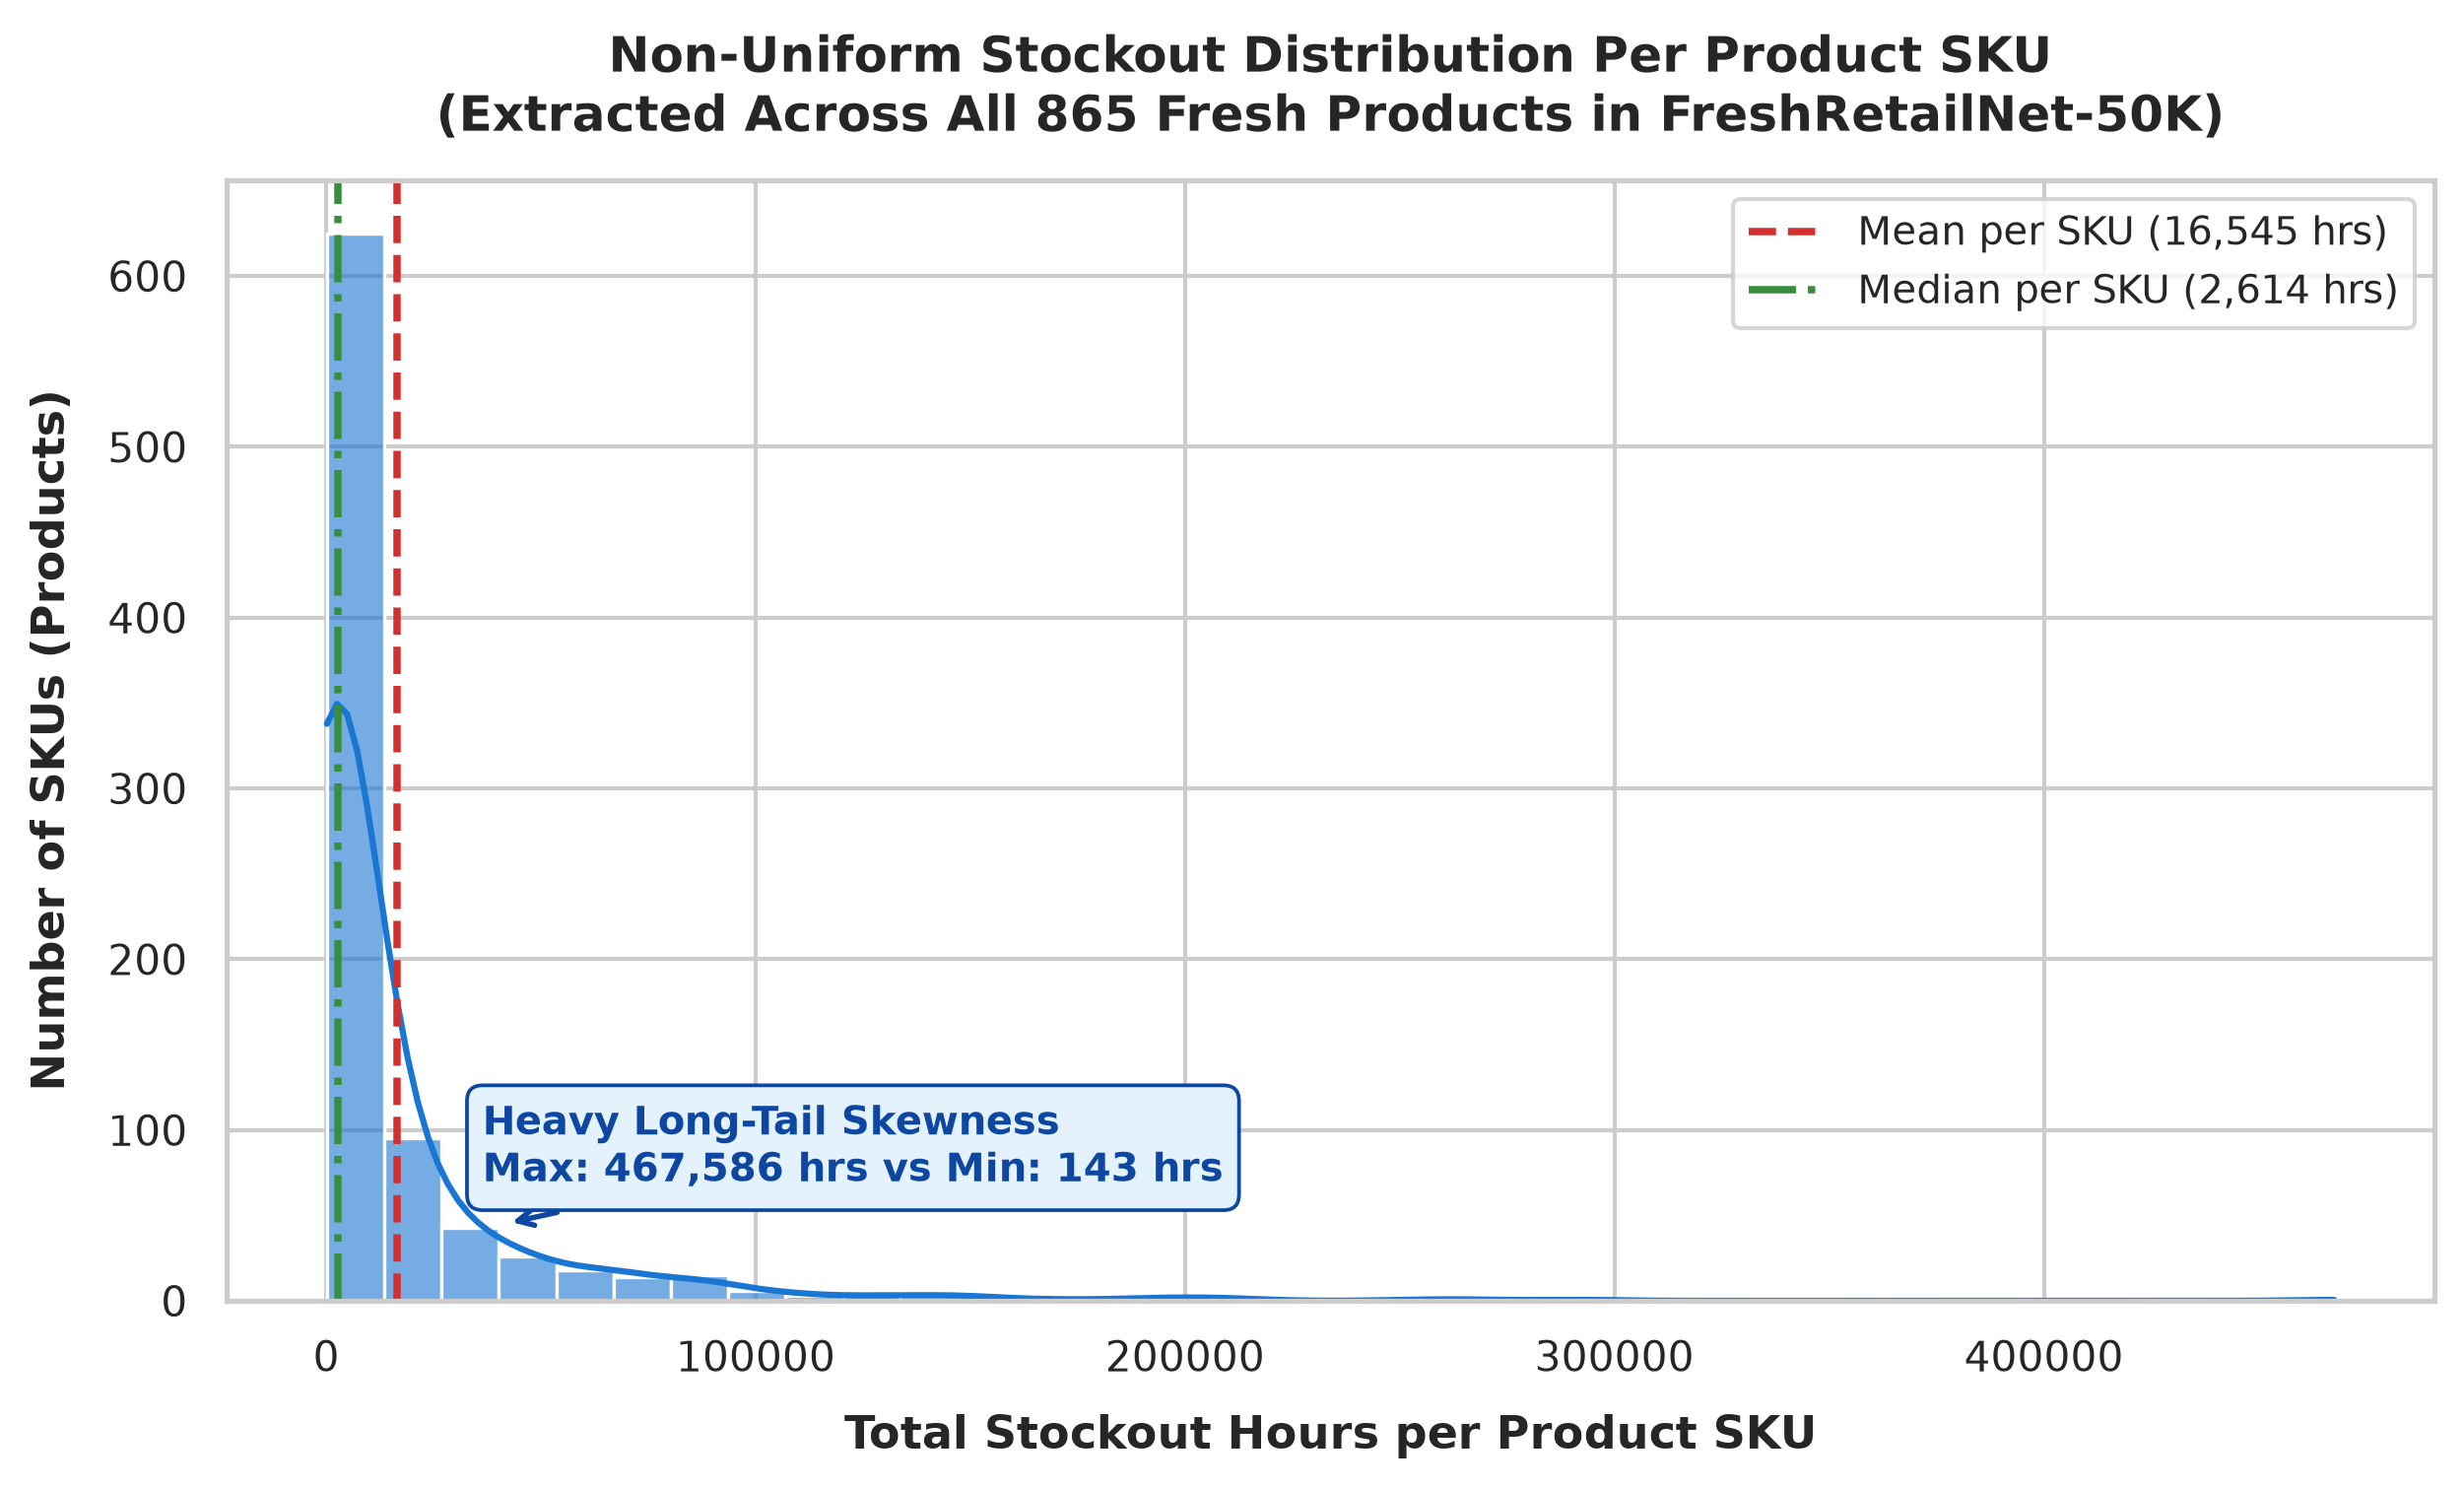
\includegraphics[width=\textwidth,height=4.6cm,keepaspectratio]{images/stockout_distribution_analysis.png}\\
      \vspace{2pt}
      \tiny{FreshRetailNet-50K Stockout Distribution across 865 SKUs}
    \end{column}
    
    \begin{column}{0.50\textwidth}
      \begin{block}{FreshRetailNet-50K Scale \& Scope}
        \small
        \begin{itemize}
          \item \textbf{Volume}: 50,000 store-product pairs across 898 stores.
          \item \textbf{Timeframe}: 90-day series of granular hourly data (75d Train / 15d Val).
          \item \textbf{Feature Types}: Includes sales history, stockout status, promotions, weather metrics, calendar signals, and momentum streaks.
        \end{itemize}
      \end{block}
      
      \begin{exampleblock}{Why We Selected This Dataset}
        \small
        \begin{itemize}
          \item \textbf{Pioneering Benchmark}: Designed for \textbf{censored demand estimation} in fresh retail (where out-of-stock items hide true demand).
          \item \textbf{Targeted Selection}: Isolated the \textbf{Top 15 SKUs} using a custom ranking formula to focus on high-impact goods and eliminate noise.
        \end{itemize}
      \end{exampleblock}
    \end{column}
  \end{columns}
\end{frame}

% ==========================================
% SLIDE 6: INITIAL BENCHMARK: LSTM VS TRANSFORMERS VS RNNS
% ==========================================
\begin{frame}{Model Family Comparison: Simple LSTMs Beat Heavy Transformers}
  \begin{columns}[c]
    \begin{column}{0.58\textwidth}
      \centering
      \vspace{12pt}
      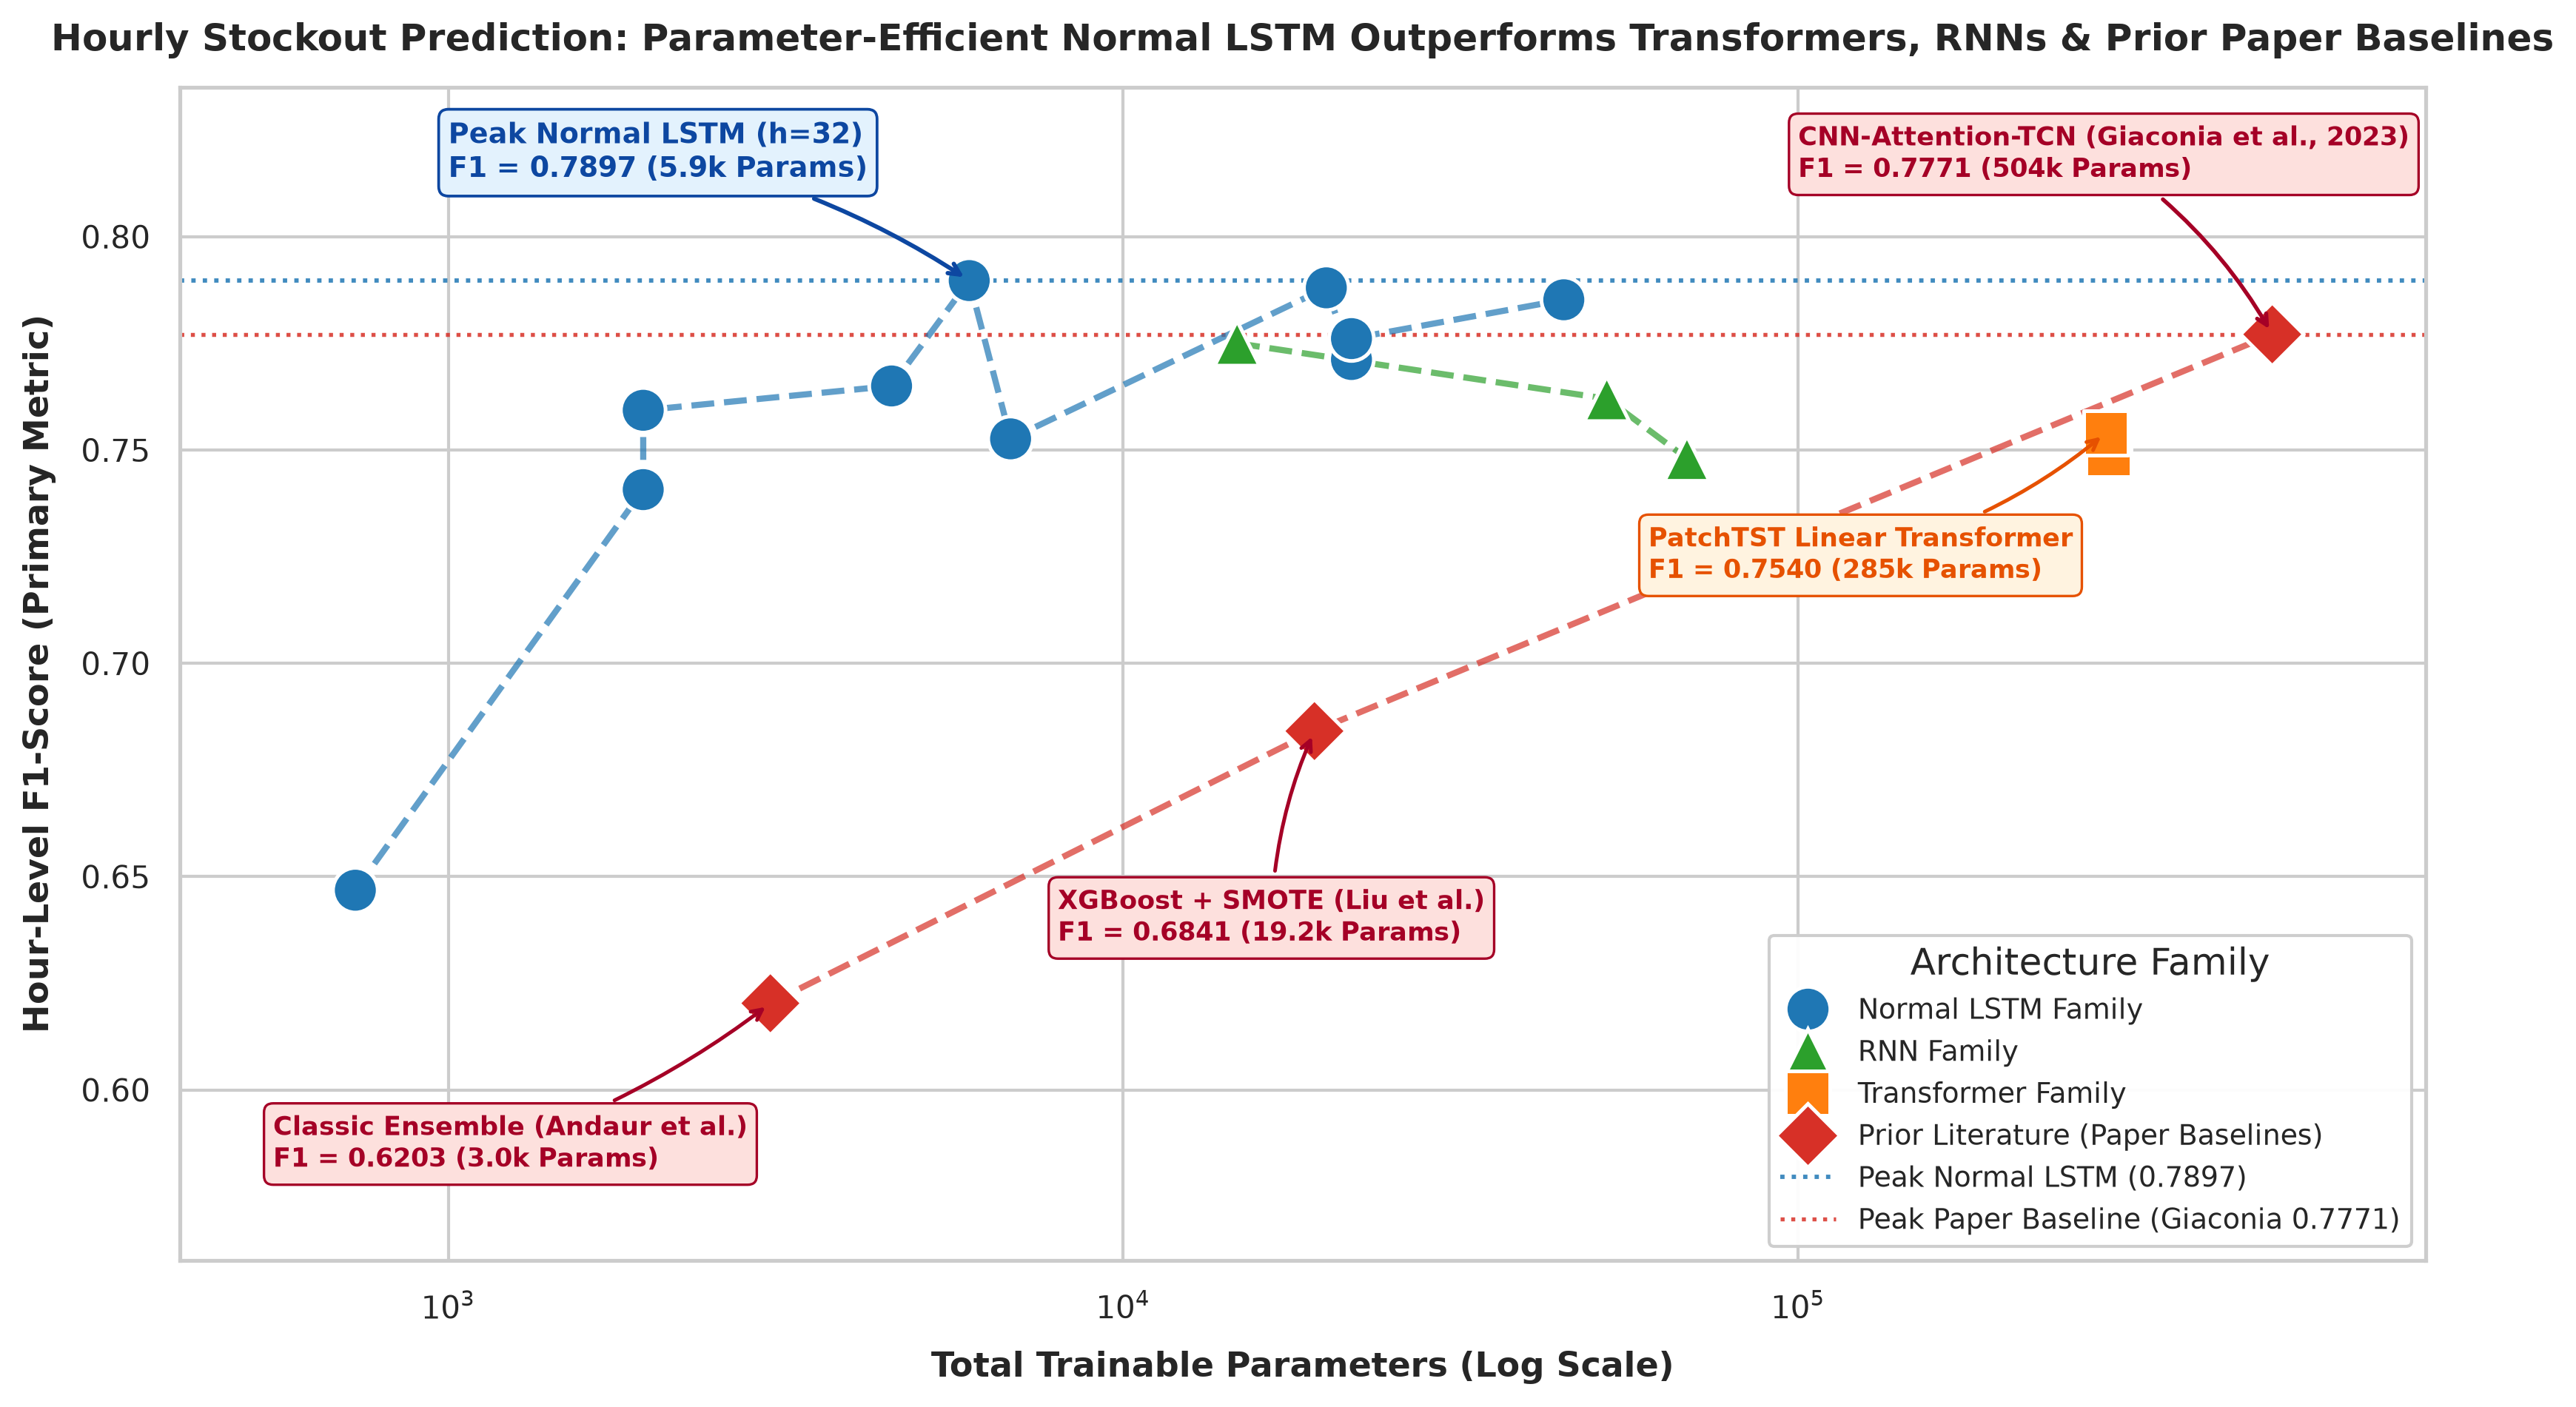
\includegraphics[width=\textwidth]{images/hourly_f1_vs_params_by_family.png}
    \end{column}
    
    \begin{column}{0.40\textwidth}
      \begin{block}{Key Empirical Findings}
        \begin{itemize}
          \item \textbf{Parameter Efficiency}: Normal LSTMs (5.9k--44.9k params) reach \textbf{0.7852--0.7897 F1-Score}, matching or beating heavy Transformers.
          \item \textbf{Transformer Overparameterization}: PatchTST (285k params) \& TFT (288k params) peak at \textbf{0.7540--0.7685 F1-Score}.
          \item \textbf{Why LSTMs Win}: Sequential state memory $h_t$ naturally aligns with continuous hourly depletion better than permutation-invariant self-attention.
        \end{itemize}
      \end{block}
    \end{column}
  \end{columns}
\end{frame}

% ==========================================
% SLIDE 7: ML EXPLAINABILITY & IG ANALYSIS
% ==========================================
\begin{frame}{ML Explainability \& Baseline Limitations}
  \begin{columns}[T]
    \begin{column}{0.53\textwidth}
      \centering
      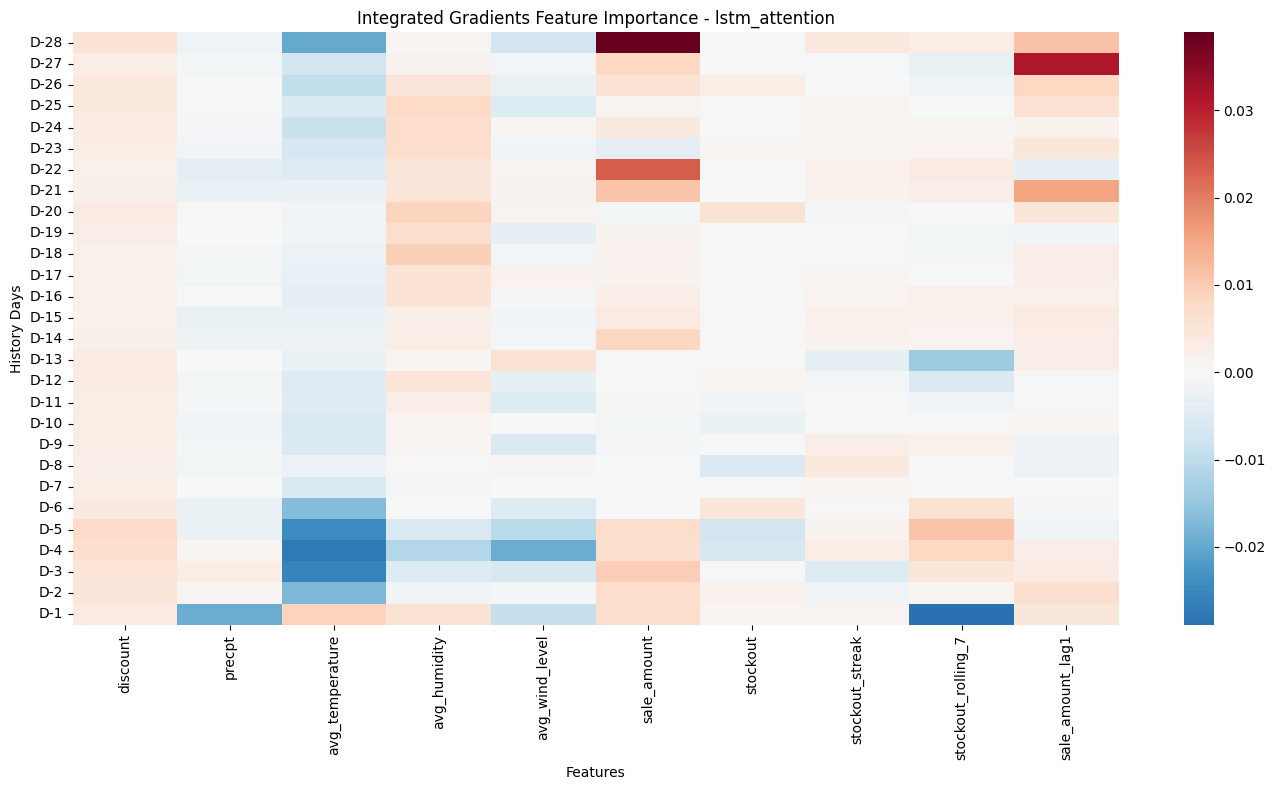
\includegraphics[width=\textwidth,height=4.5cm,keepaspectratio]{images/ig_heatmap.png}\\
      \vspace{1pt}
      \tiny{Attribution heatmap: 11-feature baseline (D-1 = most recent)}
    \end{column}
    \begin{column}{0.45\textwidth}
      \centering
      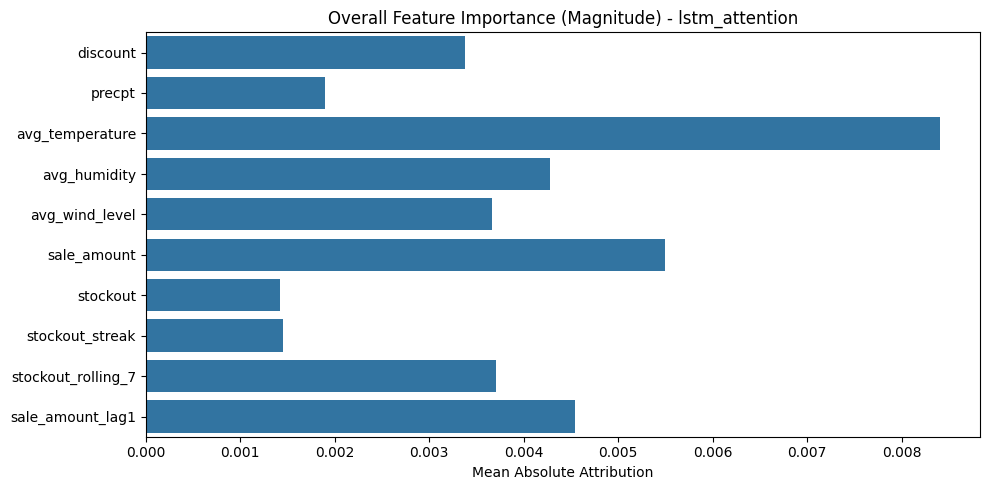
\includegraphics[width=\textwidth,height=4.5cm,keepaspectratio]{images/ig_barplot.png}\\
      \vspace{1pt}
      \tiny{Feature importance: top 6 (highlighted) outrank remaining 5}
    \end{column}
  \end{columns}
  
  \vspace{3pt}
  \begin{exampleblock}{\scriptsize Motivation for Dual-Stream Architecture}
    \scriptsize
    \begin{itemize}
      \item \textbf{F1 Plateau:} Baseline LSTM peaks at $\sim$0.789 F1; simply scaling parameters yields no gain.
      \item \textbf{Interference:} Sharing a single hidden state $h_t$ creates potential for demand/inventory interference.
      \item \textbf{IG Analysis:} Absolute attribution reveals distinct temporal behaviors for demand vs. inventory.
    \end{itemize}
    \vspace{-1pt}
    These findings motivate processing both streams independently before a task-specific fusion layer.
  \end{exampleblock}
\end{frame}

% Slide deleted and merged into previous slide
% ==========================================
% SLIDE 9: DUAL-STREAM INVENTORY SHORTCUT LSTM
% ==========================================
\begin{frame}{Our Fix: Dual-Stream Inventory Shortcut LSTM}
  \begin{columns}[c]
    \begin{column}{0.58\textwidth}
      \centering
      \includegraphics[width=\textwidth,height=5.2cm,keepaspectratio]{architecture.jpeg}\\
      \vspace{1pt}
      \tiny{Dual-Stream: Demand LSTM + Inventory LSTM + Day-14 Shortcut}
    \end{column}
    \begin{column}{0.38\textwidth}
      \centering
      \includegraphics[width=\textwidth,height=5.2cm,keepaspectratio]{images/dualstream_vs_normal_lstm_comparison.png}\\
      \vspace{1pt}
      \tiny{Architectural Impact: Dual Stream LSTM}
    \end{column}
  \end{columns}
  
  \vspace{4pt}
  \begin{exampleblock}{Key Results}
    \footnotesize
    \begin{itemize}
      \item \textbf{Inventory Shortcut}: F1 \textbf{0.7926}, MAE \textbf{3.97 hrs} at just 4,600 params.
      \item Decoupled streams consistently beat all baseline LSTM sizes.
    \end{itemize}
  \end{exampleblock}
\end{frame}

% ==========================================
% SLIDE 9: EXPLORING LINEAR DECOMPOSITION: DLINEAR
% ==========================================
\begin{frame}{Exploring Linear Decomposition: DLinear Models}
  \begin{block}{Why Explore Linear Decomposition?}
    DLinear (Zeng et al., 2023) demonstrated that single-layer linear models decomposing time series into Trend and Seasonal components can outperform complex deep networks.
  \end{block}

  \begin{columns}[T]
    \begin{column}{0.48\textwidth}
      \begin{block}{DLinear Series Decomposition}
        $$X_{\text{trend}} = \text{AvgPool}(X), \quad X_{\text{seasonal}} = X - X_{\text{trend}}$$
        $$\mathbf{Y}_{\text{pred}} = W_{\text{trend}} X_{\text{trend}} + W_{\text{seasonal}} X_{\text{seasonal}}$$
      \end{block}
    \end{column}
    
    \begin{column}{0.48\textwidth}
      \begin{block}{Standard DLinear Performance}
        \begin{itemize}
          \item \textbf{Parameters}: 6,768 parameters.
          \item \textbf{Validation F1-Score}: \textbf{0.7932}
            \begin{itemize}
              \item Outperforms Normal LSTMs (\textbf{0.7897})
              \item Outperforms Enhanced LSTMs (\textbf{0.7926})
              \item Outperforms Transformers (\textbf{0.7540})
            \end{itemize}
          \item \textbf{Stockout Recall}: \textbf{87.44\%}.
        \end{itemize}
      \end{block}
    \end{column}
  \end{columns}
\end{frame}

% ==========================================
% SLIDE 10: ARCHITECTURAL INNOVATION 2: LINEAR DLINEAR VARIATIONS
% ==========================================
\begin{frame}{Architectural Innovation 2: Linear Changes in DLinear}
  \begin{columns}[T]
    \begin{column}{0.54\textwidth}
      \centering
      \includegraphics[width=\textwidth]{images/lstm_vs_dlinear_comparison.png}
    \end{column}
    
    \begin{column}{0.43\textwidth}
      \begin{block}{Hourly Slot-Specific Linear DLinear}
        \begin{itemize}
          \item Uses \textbf{24 dedicated linear heads} ($W_1, \dots, W_{24}$) for each operational hour.
          \item Resolves inter-hour gradient conflict between morning and evening rush hours.
          \item Boosts F1 to \textbf{0.8058} (+0.0161 over LSTM).
        \end{itemize}
      \end{block}
      
      \begin{block}{Multi-Kernel Linear DLinear}
        \begin{itemize}
          \item Multi-scale moving average trend pooling ($k \in \{3, 5, 7\}$).
          \item Reaches \textbf{0.8131 F1-Score} with pure linear decomposition (13.5k params).
        \end{itemize}
      \end{block}
    \end{column}
  \end{columns}
\end{frame}

% ==========================================
% SLIDE 11: ARCHITECTURAL INNOVATION 3: NON-LINEAR DLINEAR MODELS
% ==========================================
\begin{frame}{Architectural Innovation 3: Introducing Non-Linearity into DLinear}
  \begin{columns}[T]
    \begin{column}{0.54\textwidth}
      \centering
      \includegraphics[width=\textwidth]{images/nonlinear_dlinear_comparison.png}
    \end{column}
    
    \begin{column}{0.43\textwidth}
      \begin{block}{Non-Linear Activation Bottleneck}
        Adds GELU activation bottlenecks between decomposition and output projections:
        $$\hat{Y} = W_{\text{trend}, 2} \text{GELU}(W_{\text{trend}, 1} X_{\text{trend}}) + \text{Seasonal}$$
      \end{block}
      
      \begin{block}{Breakthrough Results}
        \begin{itemize}
          \item \textbf{Non-Linear GELU DLinear}: Reaches \textbf{91.37\% Stockout Recall} (Highest in Repo!) and \textbf{0.8083 F1}.
          \item \textbf{Multi-Kernel Non-Linear DLinear}: Reaches \textbf{0.8156 F1-Score} (New Peak F1 \& lowest 3.75h MAE).
        \end{itemize}
      \end{block}
    \end{column}
  \end{columns}
\end{frame}

% ==========================================
% SLIDE 12: COMPARATIVE ANALYSIS
% ==========================================
\begin{frame}{Comparative Analysis}
  \centering
  \small
  \begin{tabular}{llccccc}
    \toprule
    \textbf{Rank} & \textbf{Architecture Name} & \textbf{Category} & \textbf{Params} & \textbf{F1-Score} & \textbf{Recall} & \textbf{MAE (hrs)} \\
    \midrule
    \rowcolor{green!15} \textbf{1} & \textbf{Multi-Kernel Non-Linear DLinear} & Non-Linear DLinear & 42,339 & \textbf{0.8156} & 87.13\% & \textbf{3.75} \\
    \rowcolor{green!10} \textbf{2} & \textbf{Multi-Kernel Linear DLinear} & Linear (Multi-Scale) & 13,539 & \textbf{0.8131} & 85.22\% & 3.86 \\
    \rowcolor{green!5} \textbf{3} & \textbf{Non-Linear GELU DLinear} & Non-Linear DLinear & 21,168 & \textbf{0.8083} & \textbf{91.37\%} & 4.20 \\
    4 & Hourly Slot-Specific DLinear & Linear (24 Heads) & 6,744 & \textbf{0.8058} & 88.02\% & 4.23 \\
    5 & Standard Linear DLinear & Linear (Decomp) & 6,768 & \textbf{0.7932} & 87.44\% & 4.28 \\
    6 & Dual-Stream Inventory Shortcut & LSTM Family & 4,600 & \textbf{0.7926} & 80.79\% & 3.96 \\
    \rowcolor{blue!10} 7 & Best Normal LSTM (h=32) & Normal LSTM & 5,912 & \textbf{0.7897} & 81.29\% & 4.31 \\
    8 & Feature-Reduced Standard LSTM & Normal LSTM & 19,992 & 0.7880 & 81.60\% & 4.58 \\
    9 & Baseline Standard LSTM (h=96) & Normal LSTM & 44,952 & 0.7852 & 80.40\% & 4.67 \\
    10 & CNN-Attention-TCN (Giaconia et al., 2023) & Deep CNN-TCN & 504,088 & 0.7771 & 85.45\% & 4.71 \\
    11 & Vanilla Simple RNN (h=64) & RNN Family & 14,744 & 0.7750 & 81.02\% & 4.23 \\
    12 & PatchTST Patch Linear & Transformer & 285,624 & 0.7540 & 81.90\% & 4.16 \\
    13 & XGBoost + SMOTE (Liu et al., 2025) & GBDT / Resample & 19,200 & 0.6841 & -- & -- \\
    14 & Classic Ensemble (Andaur et al., 2021) & ML Ensemble & 3,000 & 0.6203 & -- & -- \\
    \bottomrule
  \end{tabular}
\end{frame}

% ==========================================
% SLIDE 13: CONCLUSION AND FUTURE SCOPE
% ==========================================
\begin{frame}{Conclusion and Future Scope}
  \begin{columns}[T]
    \begin{column}{0.48\textwidth}
      \begin{block}{Key Conclusions}
        \begin{itemize}
          \item \textbf{Lightweight Linear Decompositions Win}: DLinear variants (13k--42k params) outperform heavy Transformers ($>280\text{k}$ params) and deep CNN-TCN models ($>500\text{k}$ params).
          \item \textbf{GELU Non-Linearity Bottleneck}: Exceeds standard linear limits by flawlessly mapping sudden shelf-depletion step-functions, achieving a peak \textbf{0.8156 F1} and \textbf{91.37\% Recall}.
          \item \textbf{Edge-Deployable Efficiency}: Designed with a tiny parameter footprint specifically so local retail shops lacking heavy cloud infrastructure can run urgent stockout calculations on-device.
        \end{itemize}
      \end{block}
    \end{column}
    
    \begin{column}{0.48\textwidth}
      \begin{exampleblock}{Future Scope}
        \begin{itemize}
          \item Integrate explicit choice estimation to unbias true demand during zero-stock hours.
          \item Improve the architecture to directly forecast the exact quantitative future demand for products, rather than just binary stockout probabilities.
        \end{itemize}
      \end{exampleblock}
    \end{column}
  \end{columns}
\end{frame}

% ==========================================
% SLIDE 14: REFERENCES
% ==========================================
\begin{frame}{References}
  \small
  \begin{thebibliography}{99}
    \bibitem{andaur2021} Andaur et al. (2021). Classical ML Ensembles for Retail Stockout Prediction on Tabular Data.
    \bibitem{giaconia2023} Giaconia \& Chamas (2023). Deep Learning Architectures (CNN, Self-Attention, TCN) for Intraday Stockout Probability.
    \bibitem{liu2025} Liu et al. (2025). Large-Scale Imbalance Handling (XGBoost \& SMOTE) for Stockout Events.
    \bibitem{hierarchical} \textit{A Coupled Hierarchical Architecture for Multi-Granularity Demand Forecasting} (FreshRetail Benchmark).
    \bibitem{censored} \textit{When Less Data Is Better: Eliminating Stockout-Induced Bias in Choice Estimation} (FreshRetail Benchmark).
    \bibitem{zeng2023} Zeng, A., Chen, M., Zhang, L., \& Qi, Q. (2023). Are Transformers Effective for Time Series Forecasting? (DLinear).
  \end{thebibliography}
\end{frame}

\end{document}
